\documentclass{article}

\usepackage{amsmath,amssymb}
\usepackage{tikz}
\usepackage{pgfplots}
\usepackage{xcolor}
\usepackage[left=2.1cm,right=3.1cm,bottom=3cm,footskip=0.75cm,headsep=0.5cm]{geometry}
\usepackage{enumerate}
\usepackage{enumitem}
\usepackage{marvosym}
\usepackage{tabularx}
\usepackage{multirow}
\usepackage[colorlinks = true, linkcolor = blue, urlcolor  = blue, citecolor = blue, anchorcolor = blue]{hyperref}
\usepackage{ulem}

\usepackage{listings}
\definecolor{lightlightgray}{rgb}{0.95,0.95,0.95}
\definecolor{lila}{rgb}{0.8,0,0.8}
\definecolor{mygray}{rgb}{0.5,0.5,0.5}
\definecolor{mygreen}{rgb}{0,0.8,0.26}
\lstdefinestyle{java} {language=java}
\lstset{language=java,
	basicstyle=\ttfamily,
	keywordstyle=\color{lila},
	commentstyle=\color{lightgray},
	stringstyle=\color{mygreen}\ttfamily,
	backgroundcolor=\color{white},
	showstringspaces=false,
	numbers=left,
	numbersep=10pt,
	numberstyle=\color{mygray}\ttfamily,
	identifierstyle=\color{blue},
	xleftmargin=.1\textwidth, 
	%xrightmargin=.1\textwidth,
	escapechar=§,
}

\usepackage[utf8]{inputenc}

\renewcommand*{\arraystretch}{1.4}

\newcolumntype{L}[1]{>{\raggedright\arraybackslash}p{#1}}
\newcolumntype{R}[1]{>{\raggedleft\arraybackslash}p{#1}}
\newcolumntype{C}[1]{>{\centering\let\newline\\\arraybackslash\hspace{0pt}}m{#1}}

\newcommand{\E}{\mathbb{E}}
\DeclareMathOperator{\rk}{rk}
\DeclareMathOperator{\Var}{Var}
\DeclareMathOperator{\Cov}{Cov}
\DeclareMathOperator{\SD}{SD}
\DeclareMathOperator{\Cor}{Cor}

\title{\textbf{Mensch-Computer-Interaktion, Übung 4}}
\author{\textsc{Henry Haustein}, \textsc{Dennis Rössel}}
\date{}

\begin{document}
	\maketitle
	
	\section*{Aufgabe 4.1: Open Card Sorting durchführen}
	\begin{enumerate}[label=(\alph*)]
		\item Post-It-Begriffe: Dokument hochladen, Frage stellen, Antwort hinzufügen, nach Dokumenten suchen, Antwort liken, Profil ansehen, eigenes Profil bearbeiten, Kurse suchen, Kursen beitreten, Dokument herunterladen
		\item gefundene Gruppen:
		\begin{itemize}
			\item Dokumente: Dokument hochladen, nach Dokumenten suchen, Dokument herunterladen
			\item Profil: Profil bearbeiten, Profil ansehen
			\item Interaktion: Frage stellen, Antwort hinzufügen, Antwort liken
			\item Kurse: Kurse suchen, Kursen beitreten
		\end{itemize}
	\end{enumerate}

	\section*{Aufgabe 4.2: Lo-Fi-Prototyp erstellen}
	 Startseite
	 \begin{center}
	 	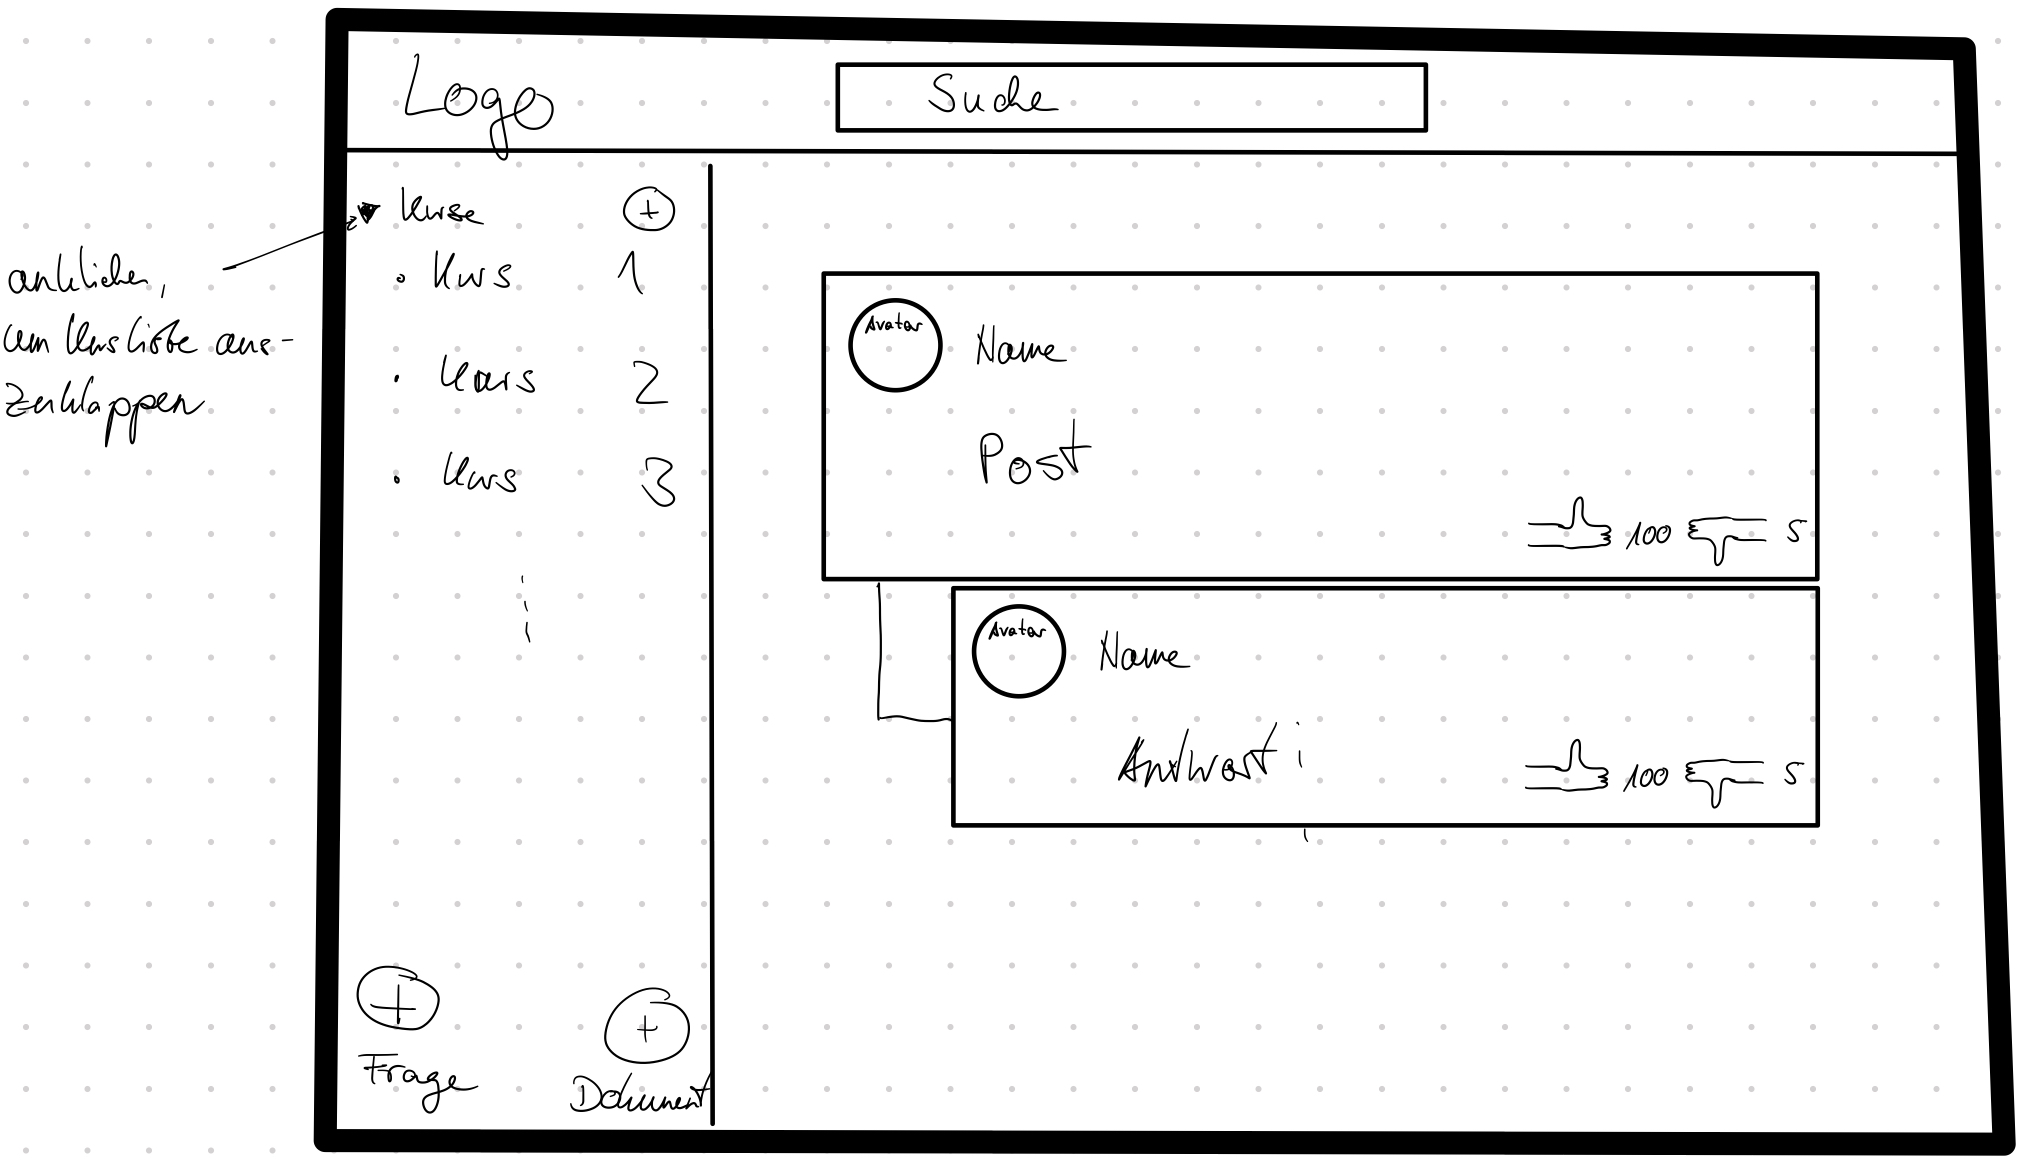
\includegraphics[scale=0.15]{startseite.jpeg}
	 \end{center}
 	\pagebreak
 	Profil
 	\begin{center}
 		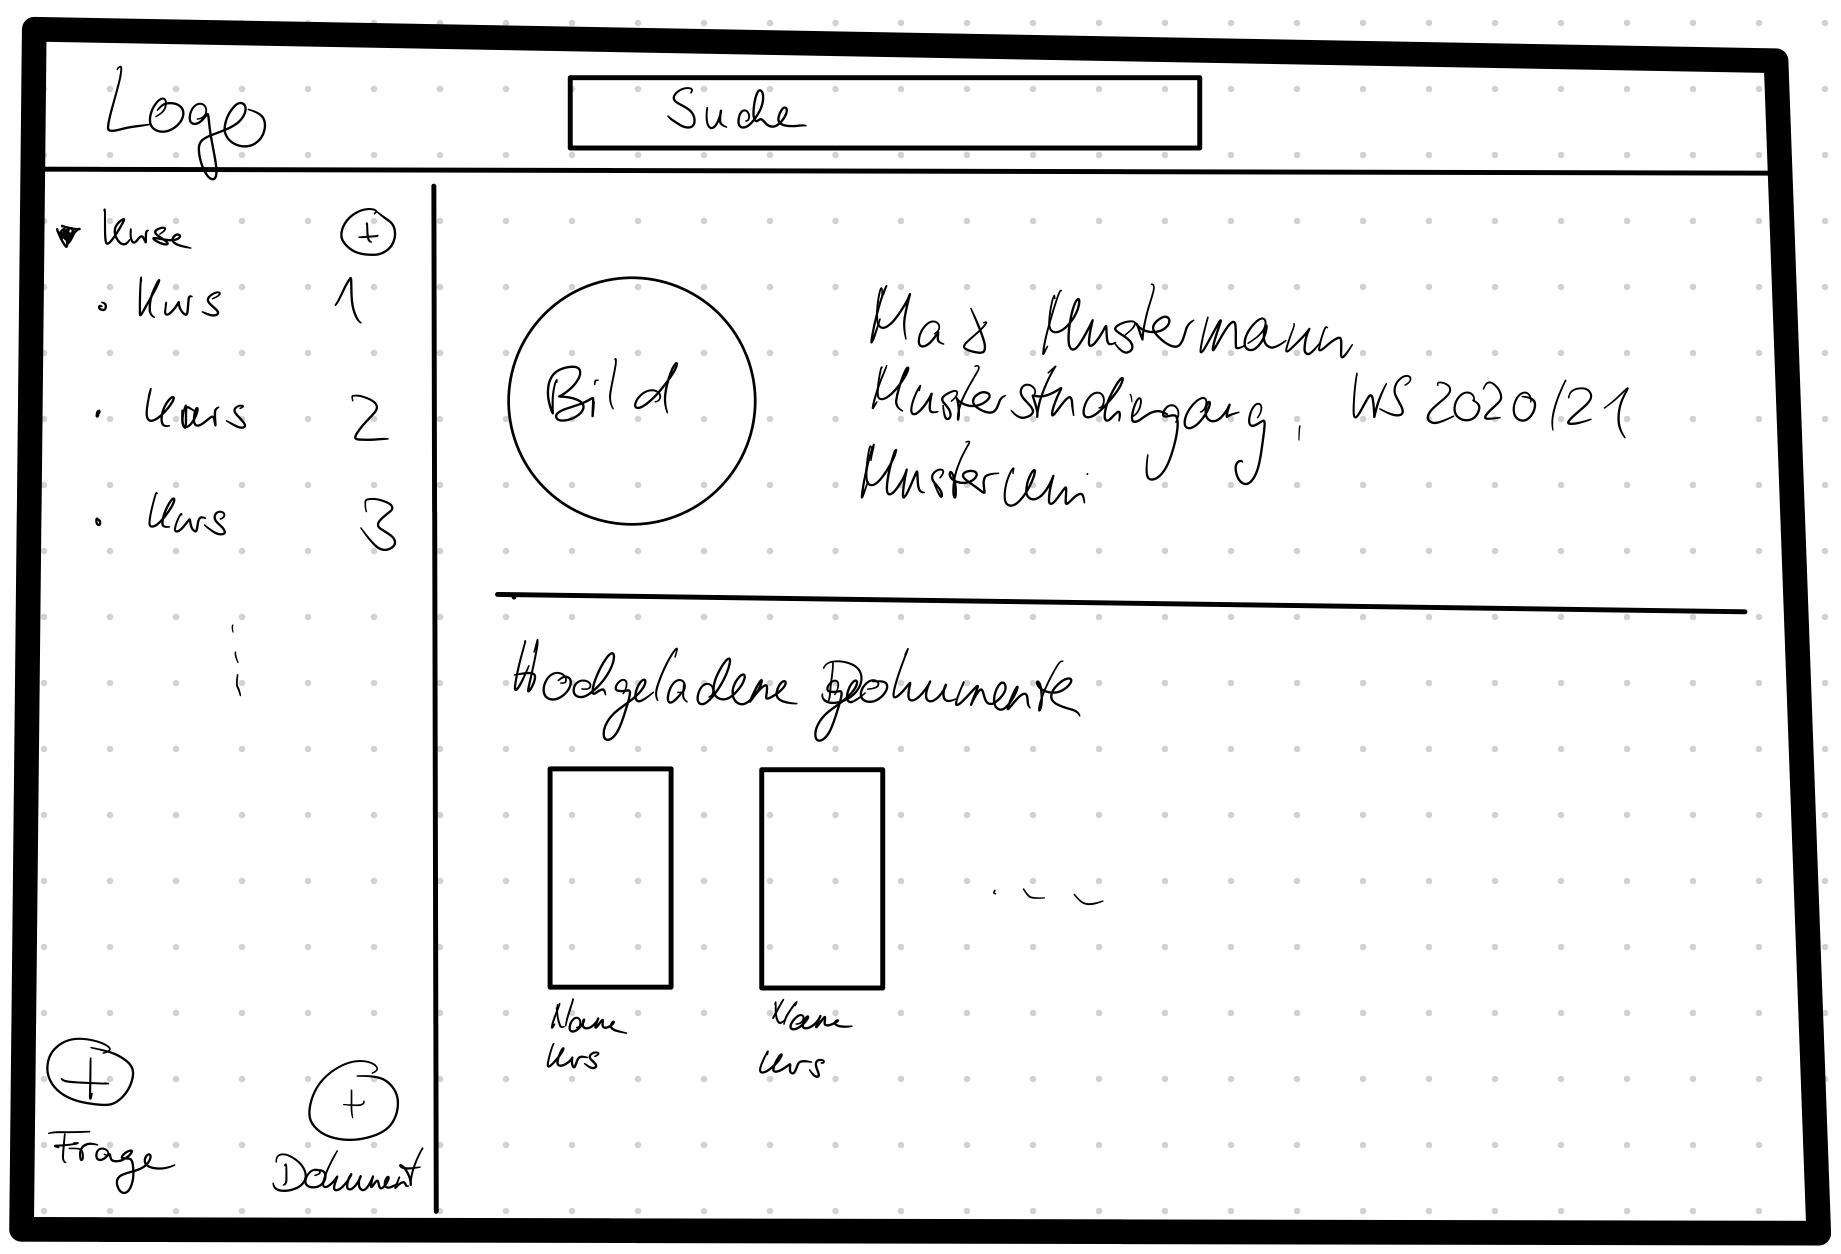
\includegraphics[scale=0.15]{profil.jpeg}
	 \end{center}
 	Dokument
 	\begin{center}
 		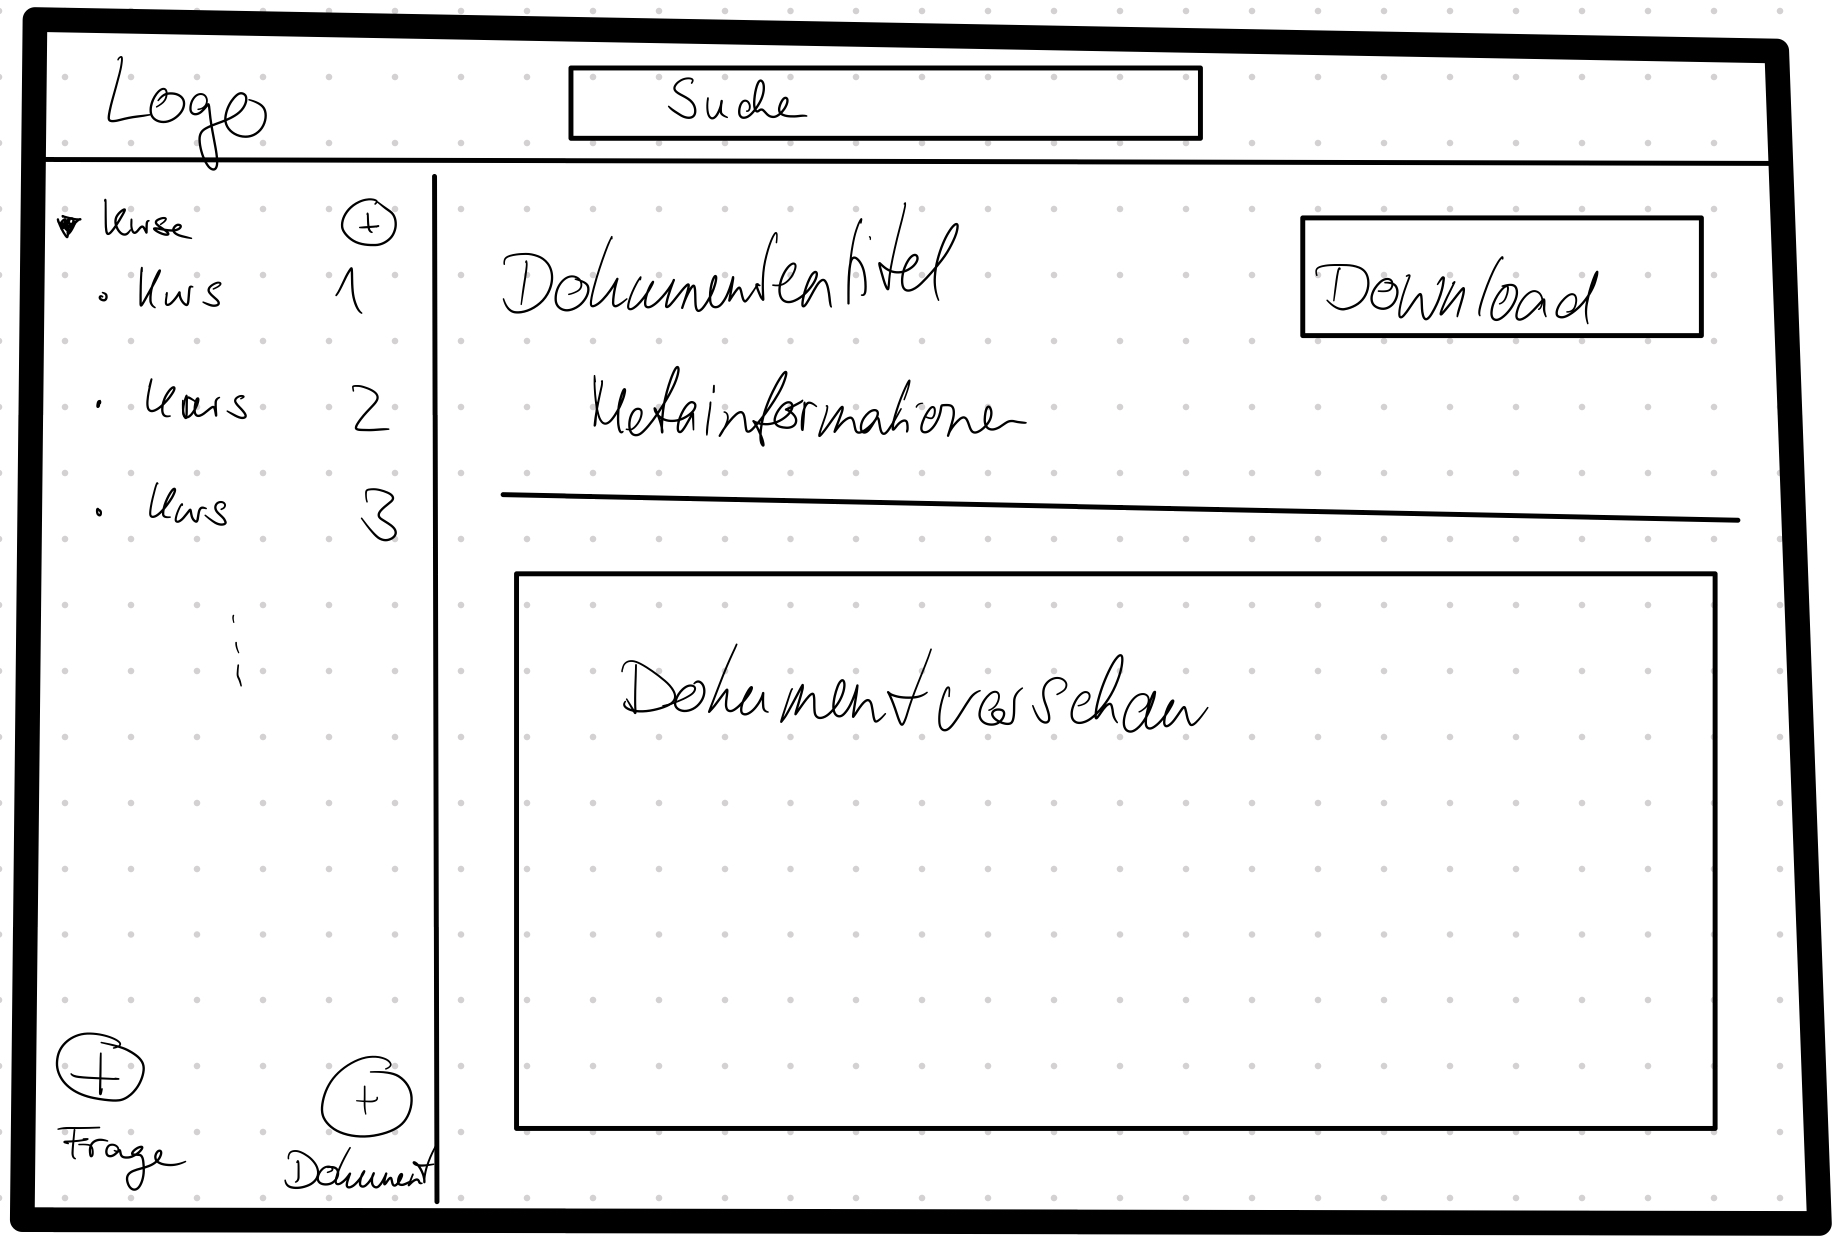
\includegraphics[scale=0.15]{dokument.jpeg}
 	\end{center}
 
 	\section*{Aufgabe 4.3: Statechart erstellen}
 	\begin{center}
 		\includegraphics[scale=0.5]{statemaschine.png}
 	\end{center}
	
\end{document}